%%%%%%%%%%%%%%%%%%%%%%%%%%%%%%%%%%%%%%%%%%%%%%%%%%%%%%%%%%%%%%%%%%%%%%%%%%%%%%%%
%2345678901234567890123456789012345678901234567890123456789012345678901234567890
%        1         2         3         4         5         6         7         8

\documentclass[letterpaper, 10 pt, conference]{ieeeconf}  % Comment this line out
                                                          % if you need a4paper
%\documentclass[a4paper, 10pt, conference]{ieeeconf}      % Use this line for a4
                                                          % paper

\IEEEoverridecommandlockouts                              % This command is only
                                                          % needed if you want to
                                                          % use the \thanks command
\overrideIEEEmargins
% See the \addtolength command later in the file to balance the column lengths
% on the last page of the document



% The following packages can be found on http:\\www.ctan.org
\usepackage{graphics} % for pdf, bitmapped graphics files
\usepackage{epsfig} % for postscript graphics files
%\usepackage{mathptmx} % assumes new font selection scheme installed
%\usepackage{times} % assumes new font selection scheme installed
\usepackage{amsmath} % assumes amsmath package installed
\usepackage{amssymb}  % assumes amsmath package installed

% Added packages.
\usepackage{float}
\usepackage{listings}
\usepackage{chngcntr}
\usepackage{color} %red, green, blue, yellow, cyan, magenta, black, white
\definecolor{codegreen}{rgb}{0,0.6,0}
\definecolor{codegray}{rgb}{0.5,0.5,0.5}
\definecolor{codepurple}{rgb}{0.58,0,0.82}
\definecolor{mygreen}{RGB}{28,172,0} 
\definecolor{mylilas}{RGB}{170,55,241}
\definecolor{backcolour}{rgb}{0.95,0.95,0.92}


\lstset{language=Matlab,
    basicstyle=\color{black} \small,
    breaklines=true,
    morekeywords={matlab2tikz},
    keywordstyle=\color{blue},
    morekeywords=[2]{1},
    keywordstyle=[2]{\color{black}},
    identifierstyle=\color{black},
    stringstyle=\color{mylilas},
    commentstyle=\color{mygreen},
    showstringspaces=false,% Without this there will be a symbol in the places where there is a space
    numbers=left, % Number Location relative to code
    numberstyle={\small \color{black}},% Size and color of the line numbers
    numbersep=-9pt, % This defines how far the numbers are from the text
    emph=[1]{for,end,break},
    emphstyle=[1]\color{red}, % Some words to emphasise
    breaklines=true, % Allows comments to wrap automatically
    postbreak=\mbox{\textcolor{red}{$\hookrightarrow$}\space} % Places red arrow to hightlight break
}
% End added packages.
\PassOptionsToPackage{hyphens}{url}\usepackage{hyperref}
\usepackage{url}
\usepackage[ruled, vlined, linesnumbered]{algorithm2e}
%\usepackage{algorithm}
\usepackage{verbatim} 
%\usepackage[noend]{algpseudocode}
\usepackage{soul, color}
\usepackage{lmodern}
\usepackage{fancyhdr}
\usepackage[utf8]{inputenc}
\usepackage{fourier} 
\usepackage{array}
\usepackage{makecell}

\SetNlSty{large}{}{:}

\renewcommand\theadalign{bc}
\renewcommand\theadfont{\bfseries}
\renewcommand\theadgape{\Gape[4pt]}
\renewcommand\cellgape{\Gape[4pt]}

% IAN - Command to set arabic numerals for tables.
\renewcommand{\thetable}{\arabic{table}}
% IAN: End

\newcommand{\rework}[1]{\todo[color=yellow,inline]{#1}}

\makeatletter
\newcommand{\rom}[1]{\romannumeral #1}
\newcommand{\Rom}[1]{\expandafter\@slowromancap\romannumeral #1@}
\makeatother

\pagestyle{plain} 

\title{\LARGE \bf
Accuracy of Simple Performant Analytical Hall-effect Thruster Modeling
}

%\author{ \parbox{3 in}{\centering Huibert Kwakernaak*
%         \thanks{*Use the $\backslash$thanks command to put information here}\\
%         Faculty of Electrical Engineering, Mathematics and Computer Science\\
%         University of Twente\\
%         7500 AE Enschede, The Netherlands\\
%         {\tt\small h.kwakernaak@autsubmit.com}}
%         \hspace*{ 0.5 in}
%         \parbox{3 in}{ \centering Pradeep Misra**
%         \thanks{**The footnote marks may be inserted manually}\\
%        Department of Electrical Engineering \\
%         Wright State University\\
%         Dayton, OH 45435, USA\\
%         {\tt\small pmisra@cs.wright.edu}}
%}

\author{Ian Soledade% <-this % stops a space 
\\ Research Seminar Class \\
Boulder High School \\
1604 Arapahoe Rd, Boulder, CO 80302 \\
{\tt\small\ irsoledade01@bvsd.org} \\ \\
Mentor: Charles Lipscomb%
\\ Nonequilibrium Gas and Plasma Dynamics Laboratory \\
University of Colorado at Boulder \\
3775 Discovery Dr, Boulder, CO 80303 \\
{\tt\small charles.lipscomb@colorado.edu}
}


\begin{document}



\maketitle
\thispagestyle{plain}
\pagestyle{plain}



%%%%%%%%%%%%%%%%%%%%%%%%%%%%%%%%%%%%%%%%%%%%%%%%%%%%%%%%%%%%%%%%%%%%%%%%%%%%%%%%
\begin{abstract}

This paper discusses analytical modeling for Hall-effect thrusters (HETs). The purpose of these models is to provide a simple and efficient way to acquire boundary conditions for plume modeling, as well as some basic estimates for thruster performance. These boundary conditions include values such as the number density and ion velocity. Models were developed using symbolic computation in MATLAB to vastly cut down on the amount of human effort required to implement a new model. The development process began with a proof-of-concept model, then new models were implemented with new equations and unknowns to incorporate more of the effects regarding HET operation. Models are then tested against real-world data from the H9 HET. Preliminary results show that the analytical approach to boundary condition modeling is highly effective for thrust values, while Isp values still lack accuracy. Additionally, models get less accurate as the HET power is increased, limiting viability as current developmental focus for HETs is on increasing power.\\

\end{abstract}

\section{INTRODUCTION}

Regular rockets are a form of chemical propulsion, where a fuel is combusted, propelling the rocket forward with an explosive plume. This is how rockets have been traditionally built since their inception. However, electric propulsion is different. HETs work by ionizing an inert gas with an electron flow around an annulus-shaped exit plane, then propelling the ions forward with an electric field. Electric propulsion is much more efficient, but provides lower thrust. The high specific impulse of electric propulsiom makes it uniquely suited to a wide variety of missions such as orbit raising, stationkeeping, and interplanetary missions \cite{c3}.

A recent mission making use of electric propulsion is NASA’s Double Asteroid Redirection Test, or DART. This mission makes use of electric propulsion to change the trajectory of an asteroid. This test functioned as a proof-of-concept for a planetary defense system designed to keep the globe safe from asteroid impacts \cite{c7}. An image of DART’s impact is below:

\begin{figure}[H]
      \centering
      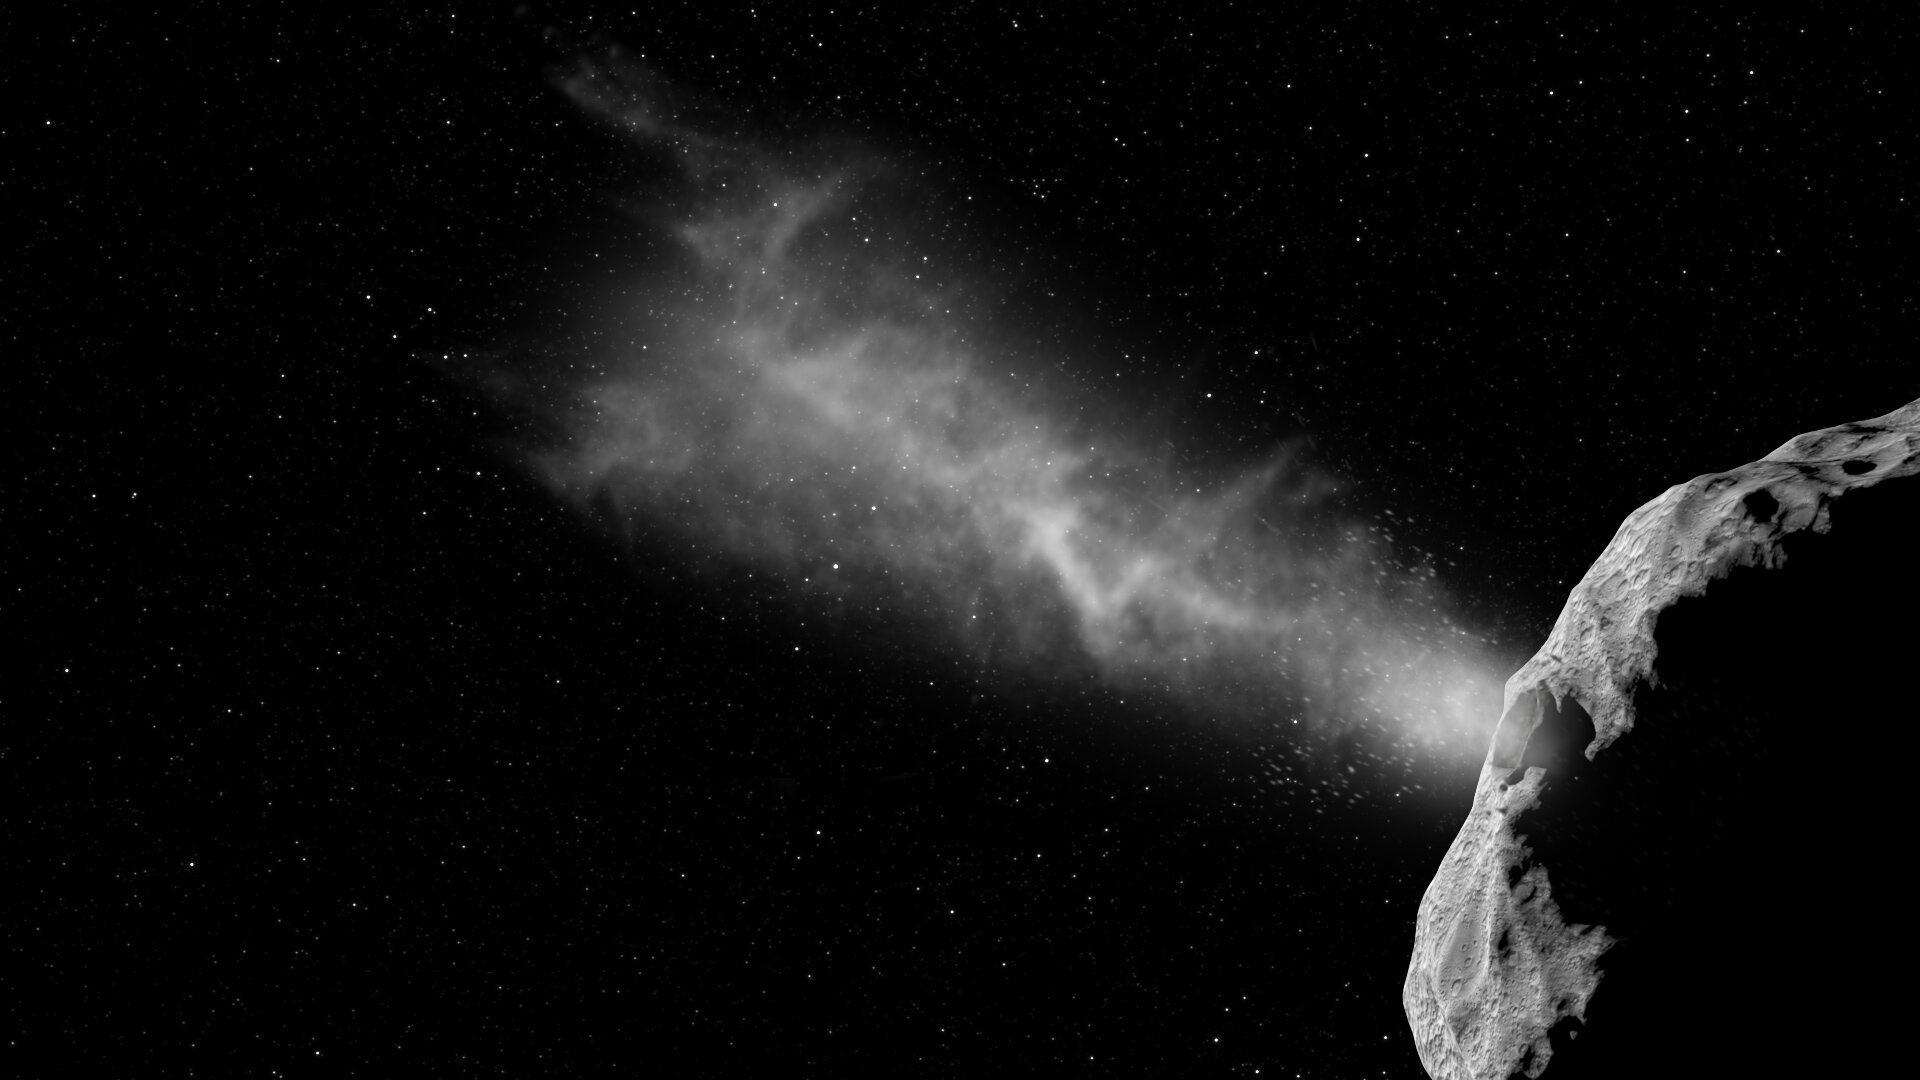
\includegraphics[width=2.5in]{Images/DART.jpg}
      \caption{DART's asteroid impact \cite{c6}.}
      \label{fig:2}
\end{figure}

Currently operational HET thruster designs are highly limited in power. These thrusters only put out power on the order of milli-Newtons, not enough for many mission sets. Therefore, organizations such as the Department of Defense and NASA are currently interested in higher power designs \cite{c3}.  The below image details the workings of a HET:

\begin{figure}[H]
      \centering
      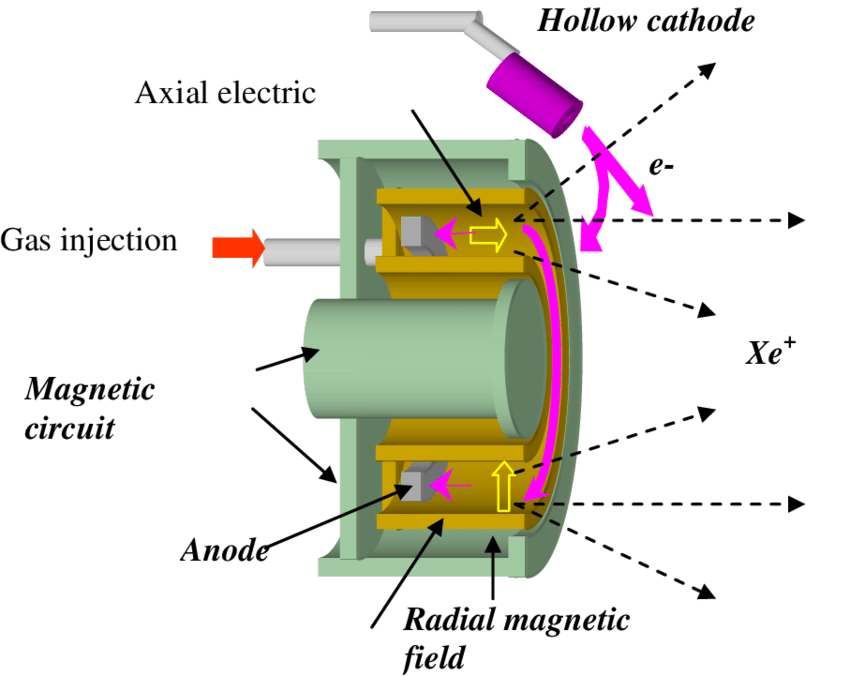
\includegraphics[width=2.5in]{Images/het_dia.png}
      \caption{Diagram of a HET \cite{c6}.}
      \label{fig:1}
\end{figure}

However, before high-power thrusters can be tested on missions, they must be tested in a vacuum chamber on Earth. Vacuum chamber testing time is quite valuable, so ensuring the operability and effectiveness of designs before testing is a must. Therefore, the ability to accurately simulate HETs is very important. These computer simulations can take a very long time to run and require special hardware. 

This research project aims to develop an analytical model for determining boundary conditions for more computationally complex HET plume models. Additionally, as these models can take time to run and require specialized hardware, having access to an accurate and reliable model for HETs that can be made and run quickly would greatly increase the speed at which HET designs can be verified for use in space. To compare the accuracy of model predictions, the H9 thruster will be used. This is because it is a modern, magnetically shielded design that is representative of those that could see use in upcoming missions \cite{c2}.

This research is not well documented in literature. Georgia Tech scientists in 2005 developed a model that hybridized numerical and analytical approaches \cite{c3}. However, this required fitting the model to data with a loss parameter, making this model thruster dependent. My approach attempts to avoid this by using a purely analytical approach, which is also far more flexible as real-world data isn’t required to develop the model.

Additionally, a NASA researcher working with CU Boulder’s Nonequilibrium Gas and Plasma Dynamics Laboratory (NGPDL) developed a similar model to this project in the early 2000s. This model is currently non-functional. However, when it is restored by the University of Colorado Boulder’s Nonequilibrium Gas and Plasma Dynamics Laboratory (NGPDL), results between this model and NGPDL’s can be compared.

\section*{NOMENCLATURE}

\begin{itemize}
    \item $T$: The effective thrust of the HET. My models are built on SI units; therefore, $T$ is measured in Newtons.
	\item $I_{sp}$: The efficiency of the thruster. Measured in seconds.
	\item $\dot{m}$: The flow rate of mass through the exit plane, written as a derivative of total mass over time. Units are kg/s.
	\item $n_a, n_i$: The number density of atoms and ions in the HET, respectively. Units are per meters cubed.
	\item $v_a, v_i$: The velocity of ions and atoms in the HET, respectively. Units are m/s.
	\item $\gamma$: The Adiabatic index, a unitless number equivalent to 5/3 for this application. Used in calculating atom speed.
	\item $k$: The amount of energy required to heat the gas used in the HET by one kelvin. Units are J/k.
	\item $m$: The mass of a single atom/ion in kg. My models all use xenon; therefore, this is equivalent to 131.29 amu.
	\item $I$: The ion beam current. Measured in amps.
	\item $A$: The area of the thruster’s annulus shaped exit plane. Measured in m2.
	\item $V_a, V_c$: The electric potentials at the anode and cathode of the HET, respectively. Measured in volts.
	\item $q$: The average charge on an ion. This is typically expressed as multiples of the fundamental charge in Coulombs.
	\item $\theta$: The average ion divergence angle. Measured in degrees.
	\item $\epsilon_0$: A constant representing the permittivity of free space. Measured in Farads per meter.
    \item $s_n$: The unitless fraction expressing the percent of ions that haave charge state $n$.
\end{itemize}

\section{MODELING PROCESS}

\subsection{Model 0:}
This model purely functioned as a proof of concept, and its outputs are hence highly inaccurate. Therefore, it is not being considered in the final data. However, it is important to talk about, as it introduces the first equations that will be used in the model. This model is built around determining 2 variables: $v_a$, the speed of sound for the inert gas used in the HET, and $n_a$, the number density of atoms in the exit plane. This information will be useful for determining other quantities later. The following equations are introduced to determine these quantities:

\begin{equation} \label{eq:1}
v_a = \sqrt{\frac{\gamma{}kT_a}{m}}
\end{equation}

\begin{equation} \label{eq:2}
\dot{m} = Amn_av_a
\end{equation}

These equations are then input into MATLAB’s equation solver to solve for the atoms’ velocity and number density. The MATLAB code to execute this task is below:

\BlankLine
\begin{lstlisting}[language=Matlab]
    syms gamma k Ta m m_dot A
    syms n a
    
    eq1 = a == sqrt(gamma * k * T / m);
    eq2 = n == m_dot / m / a / A;
    
    solution = solve([eq1, eq2], [a, n]);
    
    disp("a: " + simplify(solution.a))
    disp("n: " + simplify(solution.n))
    
    % While this code is simple, and this solution
    % could be easily found by hand, this will not
    % continue to be the case as models become pro-
    % gressively more involved. This file simply
    % shows the basic concept of using MATLAB for
    % this project.
    
\end{lstlisting}
\BlankLine

As is evident, this is a very simple task. Most of the effort for this project was processing the results of each model and running a wide variety of simulations with the resulting equations to determine model accuracy.

\subsection{Preliminary Equation Breakdown:}
There is no easy way to explain the use of the speed of sound as an accurate assumption for atom speed at the exit plane. This assumption is derived from an understanding of the Knudsen layer created by the gas flowing through the thruster. A highly simplified explanation stems from the fact that sound, by definition, cannot exist in a vacuum. Therefore, the speed of expansion of the gas into the vacuum is the speed of sound, as sound can only travel along the boundary of expansion into the surrounding environment. This explanation is highly abstract, and the true explanation requires enough research to be worthy of its own project.

The derivation of the mass flow rate equation can be accomplished with a control volume analysis. By examining flow at the exit plane boundary of the thruster, it is possible to capture an expression for mass flow rate using the below surface integral:

\begin{equation} \label{eq:3}
\dot{m}=\oiint\limits_{S}mn_a\vec{v}_a \cdot \hat{n} \,dS
\end{equation}

Evaluating this integral gives the mass flow rate equation used throughout this project.

\subsection{Model 1:}
This model is the first to attempt to describe the actual workings of a HET. This is accomplished by incorporating the effects of ions in the thruster plume. Therefore, three new equations are introduced:

\begin{equation} \label{eq:4}
E = \frac{1}{2}mv^2
\end{equation}

\begin{equation} \label{eq:5}
E = q(V_a -V_c)
\end{equation}

\begin{equation} \label{eq:6}
n_i = q(V_a -V_c)/\epsilon_0
\end{equation}

Equation \ref{eq:6} is not mathematically sound. This was an attempt to use an equality involving the derivative of electric field to find the ion number density, however, many more factors contribute to that quantity then are found in Equation \ref{eq:6}. This model does still produce relatively accurate thrust and efficiency results, as both quantities are calculated independently using the below equations, which will later be directly implemented into new models:

\begin{equation} \label{eq:7}
T = \dot{m}v_i
\end{equation}

\begin{equation} \label{eq:8}
I_{sp} = \frac{T}{\dot{m}g}
\end{equation}

The inclusion of ions in this model also requires the mass flow rate equation to use the sum of the ion and atom number densities. This requires summing two of the mass flow rate equations from Model 0, one for ions and one for atoms, to produce the actual mass flow rate:

\begin{equation} \label{eq:9}
\dot{m} = Am(n_av_a + n_iv_i)
\end{equation}

\subsection{Understanding the Use of Energy:}

As shown below in Figure \ref{fig:3}, the total potential energy of a newly introduced ion to the thruster can be readily calculated with the standard equation for potential energy due to an electric field. Additionally, due to conservation of energy, this potential energy will be equivalent to the ion’s kinetic energy after acceleration from the electric field inside the HET, another easily calculatable quantity.

\begin{figure}[H]
      \centering
      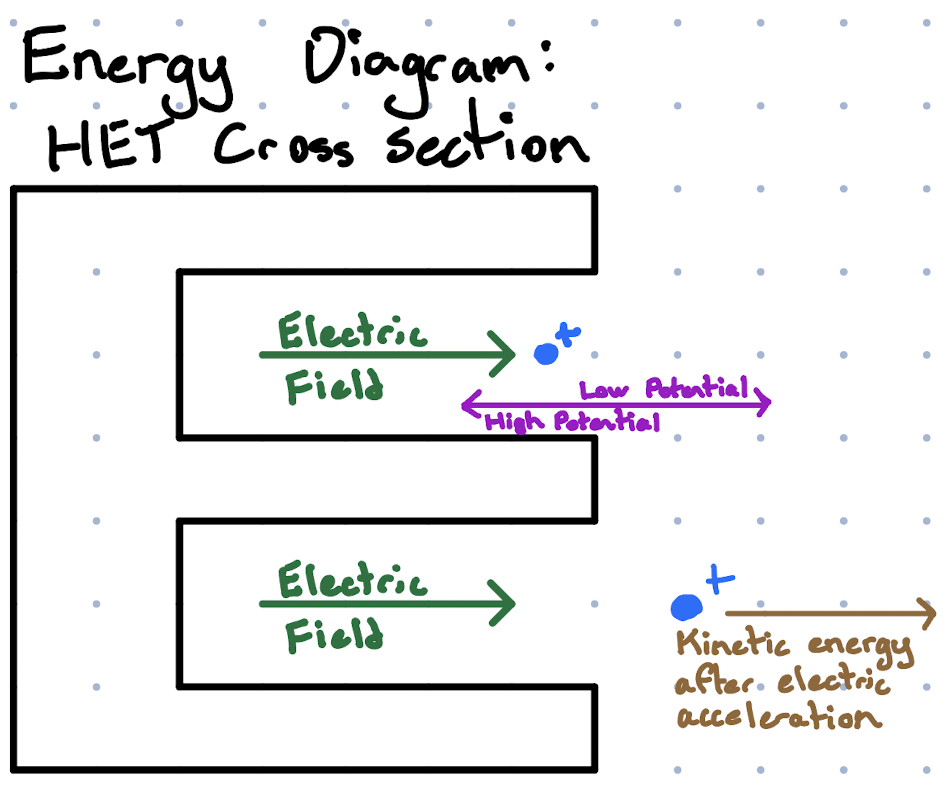
\includegraphics[width=2.5in]{Images/e_dia.png}
      \caption{Diagram of potential and kinetic energy.}
      \label{fig:3}
\end{figure}

\subsection{Models 2 and 3:}
Model 2 opts to use thrust as an input to test a solution to the incorrect ion number density equation. Therefore, Model 2 will be glossed over in favor of discussion on Model 3. Model 2 implements one equation, derived from a second control volume analysis implementing a simplified Navier-Stokes equation:

\begin{equation} \label{eq:10}
T = nmAv_i^2
\end{equation}

Model 3 fixes the issues introduced in Model 1 from the improper ion number density equation. Instead, Model 3 uses an equation for ion number density based on the HET beam current:

\begin{equation} \label{eq:11}
I = qn_iv_iA
\end{equation}

However, this means that the model has acquired another input, the beam current of the HET. This can be estimated as a fraction of the discharge current in the thruster, but this is an unreliable input. Later versions of the model will seek to rectify this. Literature states that for a Hall-effect thruster, most beam currents are around 70-80\% of the discharge current. This is a big range, and nailing these down will require a later model. For now, beam currents will be assumed at 80\%.

\subsection{Beam Current Explanation:}
Current is fundamentally an amount of charge flowing over a time interval. The ion beam current formula is built from this definition, finding the number of ions per second flowing through the exit plane. Essentially, this measures the current from the HET plume, as the ions in the plume necessarily form a current. A diagram showing this effect is below:

\begin{figure}[H]
      \centering
      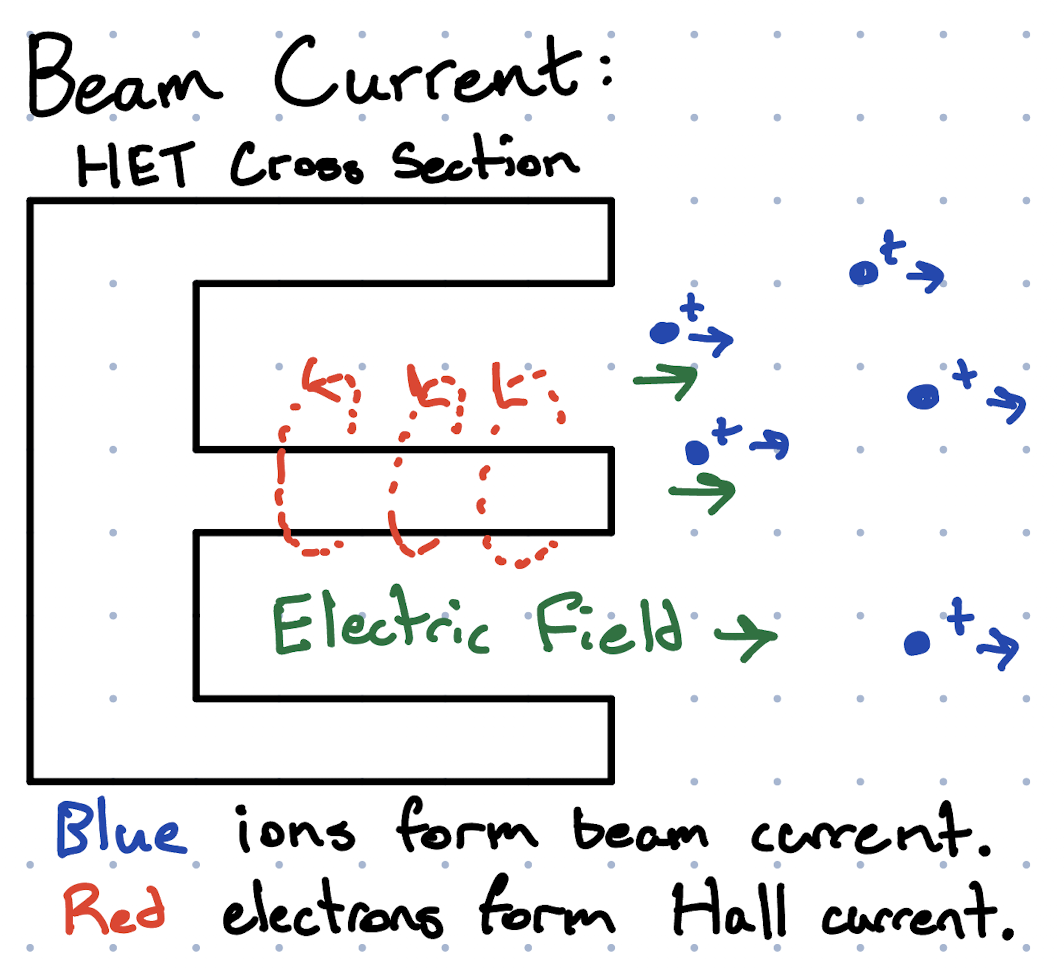
\includegraphics[width=2.5in]{Images/b_cur.png}
      \caption{Diagram showing the source of beam current.}
      \label{fig:4}
\end{figure}

\subsection{Model 4:}
This model considers the effects of multiply charged ions. This is when an atom is ionized multiple times by the Hall current in the thruster. As these ions have a higher charge, they will consequently be propelled more than their counterparts by the electric field. However, highly charged ion species are considerably rarer than ions with a simple +1 charge, as the odds of a particle being struck by electrons in the Hall current multiple times. A diagram below visualizes this effect:

\begin{figure}[H]
      \centering
      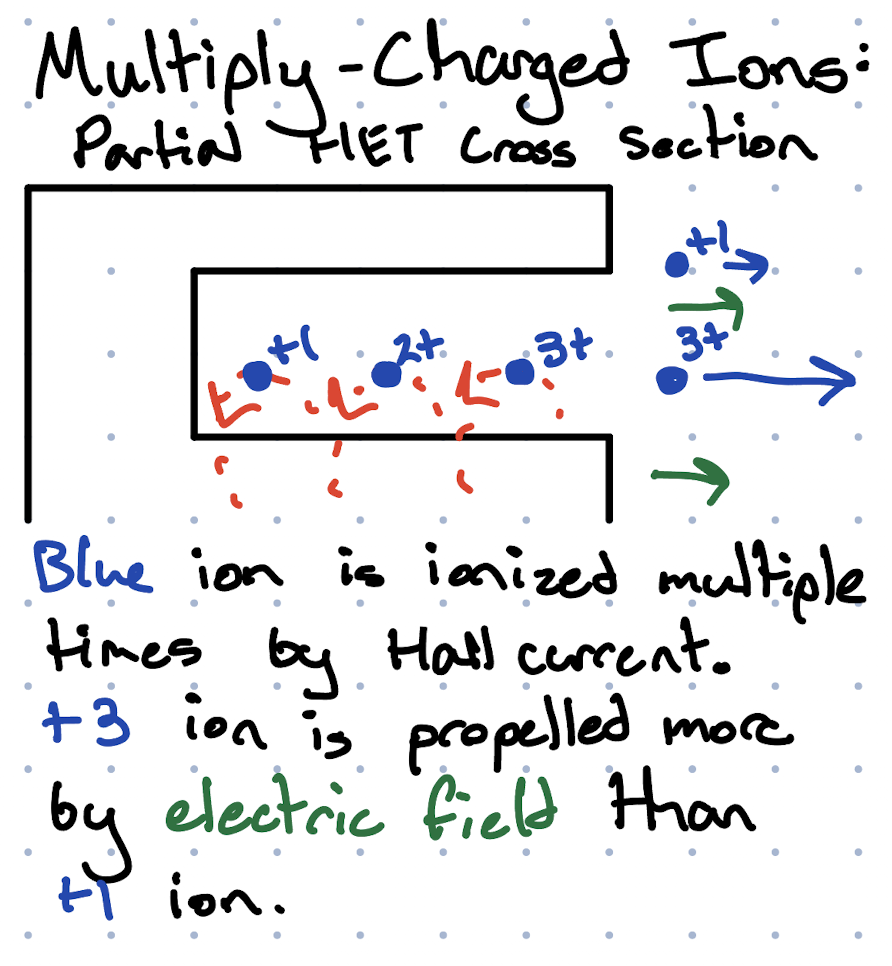
\includegraphics[width=2.5in]{Images/m_cha.png}
      \caption{Diagram displaying multiple ionization.}
      \label{fig:5}
\end{figure}

Therefore, the kinetic energy equation must be implemented three times, once for charge states +1 through +3. Any charge states beyond +3 happen so rarely as to be considered inconsequential. Additionally, the number density of ions must also be divided into number densities for each ion species. 

This does mean that there are 3 new inputs to the model, one each for the fraction of the number density that correlates to each ion species. These fractions are taken from literature \cite{c1} and will remain required inputs for all future models.

Additionally, this affects the mass flow rate equation, as now there are 3 ion species considered. This means that each species must be considered in the equation with its own number density and velocity.

Another equation that must change is the thrust equation. The easiest way to consider the effects of considering multiple species is to evaluate the thrust provided by each species independently and then sum each thrust to get a final value.

For simplicity's sake, equations requiring a change due to this model revision are listed below. An easy way to understand the required updates to the equation is to replace every statement of energy, velocity, and ion charge with its average value.

\BlankLine
List of updated equations:
\begin{itemize}
    \item Equation \ref{eq:4}
    \item Equation \ref{eq:5}
    \item Equation \ref{eq:7}
    \item Equation \ref{eq:9}
    \item Equation \ref{eq:10}
    \item Equation \ref{eq:11}
\end{itemize}

\subsection{Model 5:}
Model 5 incorporates a relatively simple change, but it marks a significant step in this process as it incorporates plume divergence, which is the final new factor of understanding a HET’s operation that will be introduced. A diagram showing the effect is below:

\begin{figure}[H]
      \centering
      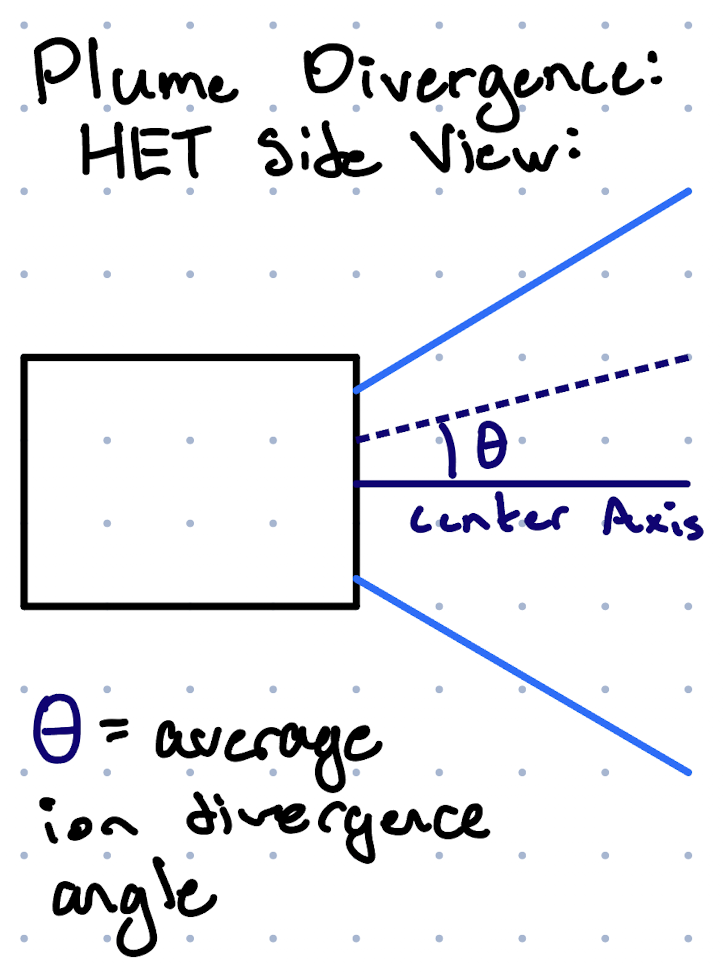
\includegraphics[width=2.2in]{Images/div.png}
      \caption{Diagram showing plume divergence.}
      \label{fig:6}
\end{figure}

While fully understanding plume divergence is quite difficult, the easiest way to consider it in a simple model design is by the average angle of divergence for any ion. For the H9 thruster, this is about 25 degrees.

This clearly decreases the thrust of a real HET, as the ion velocity takes on a horizontal component. The mass flow rate of the thruster will also decrease, as its equation is derived from a control volume analysis, which takes a surface integral in the direction of the exit plane area vector.

Therefore, the thrust equation and the mass flow rate equation must be appended with the cosine of the average ion divergence angle to compensate for this effect. The updated equations are below:

\begin{equation} \label{eq:12}
T = nmAv_i^2\cos^{2}\theta
\end{equation}

\begin{equation} \label{eq:13}
T = \dot{m}v_i\cos{\theta}
\end{equation}

\begin{equation} \label{eq:14}
\dot{m} = Am(n_av_a + n_iv_i)\cos{\theta}
\end{equation}

As this is the last major effect my models will be incorporating, future models seek to simplify and reduce the required inputs for the model to function. 

\subsection{Models 6 and 7:}
Models 6 and 7 host the same changes to the equations, however, they use a different list of inputs and outputs. Due to the nature of symbolic computation, simply shifting what variables are considered as constants will completely change how the system is solved.

While these models don’t describe anything new about the HET, it does add one more equation to the system, allowing the removal of an input. The equation implemented is actually Equation \ref{eq:13}, used previously to determine the thrust predicted by the model based on its ion velocity output(s).

Model 6 removes mass flow rate as an input, allowing the user of the model to have less data about the thruster they are attempting to simulate. Also, the internal prediction of mass flow allows some flexibility in the model to adapt to real-world losses/gains, increasing accuracy.

Model 7 instead removes the beam current. As this has been a massive unknown in previous models, removing beam current as an input allows for a massive increase in model usability. This also means that Model 7 can output a more precise beam current fraction.

Essentially, this generation of models has worked to reduce inaccuracy due to the uncertainty of inputs. This was a much-needed improvement; however, it suffers from some hidden issues. Primarily, Equations \ref{eq:12} and \ref{eq:13} are related through Equation \ref{eq:14}, meaning that the new thrust equation provides no benefit. The only reason Model 6 and Model 7 run without having an underdefined system is that the thrusts predicted by each equation are barely different, as Equation \ref{eq:12} incorporates the effects of atoms in the thrust. This slight difference in the system keeps the appearance of being fully defined enough that MATLAB can solve the system. However, this is still a mistake, so one more model is required to attempt to rectify it.

\subsection{Model 8:}
This model attempts to rectify the mistake introduced in Model 6 and Model 7 by removing model outputs to keep the system fully defined once an equation is removed. Equation \ref{eq:12} was removed due to its complexity as it was derived via control volume analysis.

As atoms have a tiny effect on the operational capabilities of the thruster, atom number density and velocity can theoretically be removed without drastically effecting model accuracy. This removes yet another equation, Equation \ref{eq:1}, as it is simply no longer needed. However, as both atom number density and velocity can be removed, the system is still fully defined. 

\section{RESULTS}

Below are graphs of model predictions against real thruster data. Additionally, tables are included showing the average percent error for each model across all tested power levels.

\begin{figure}[H]
      \centering
      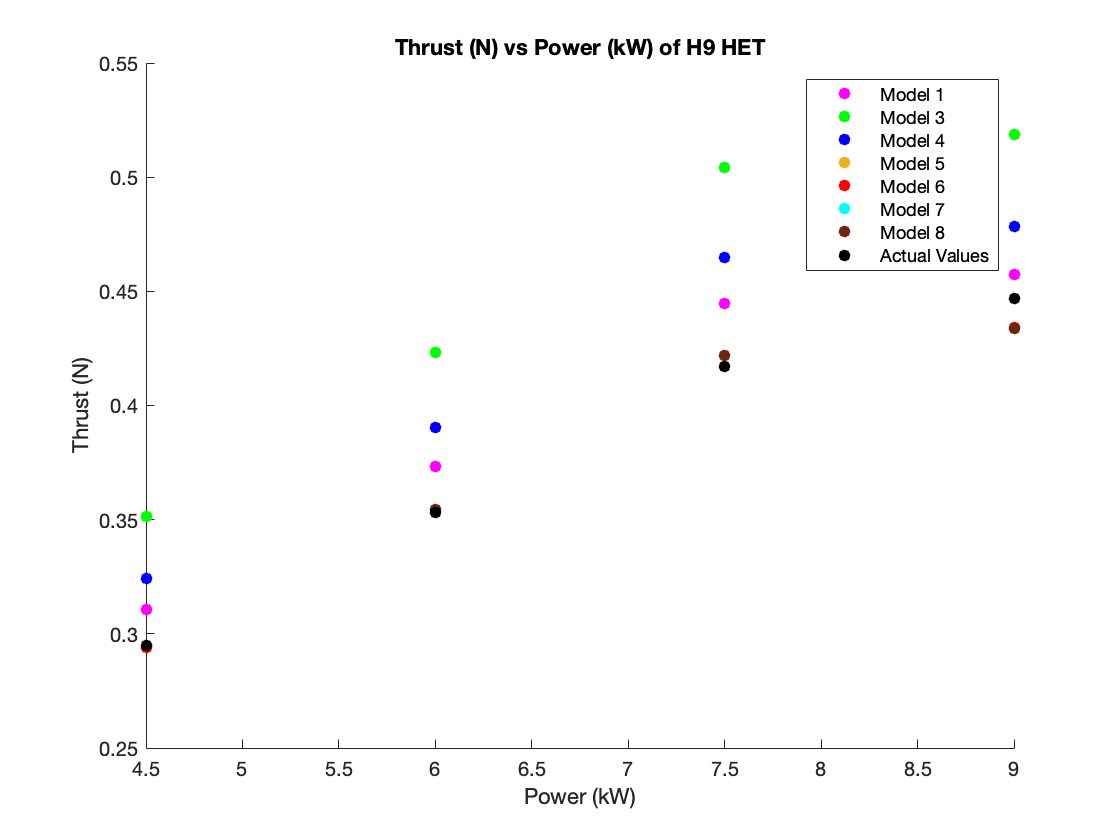
\includegraphics[width=3.3in]{Images/t_vs_p.png}
      \caption{Graph of predicted thrust values.}
      \label{fig:7}
\end{figure}

\begin{figure}[H]
      \centering
      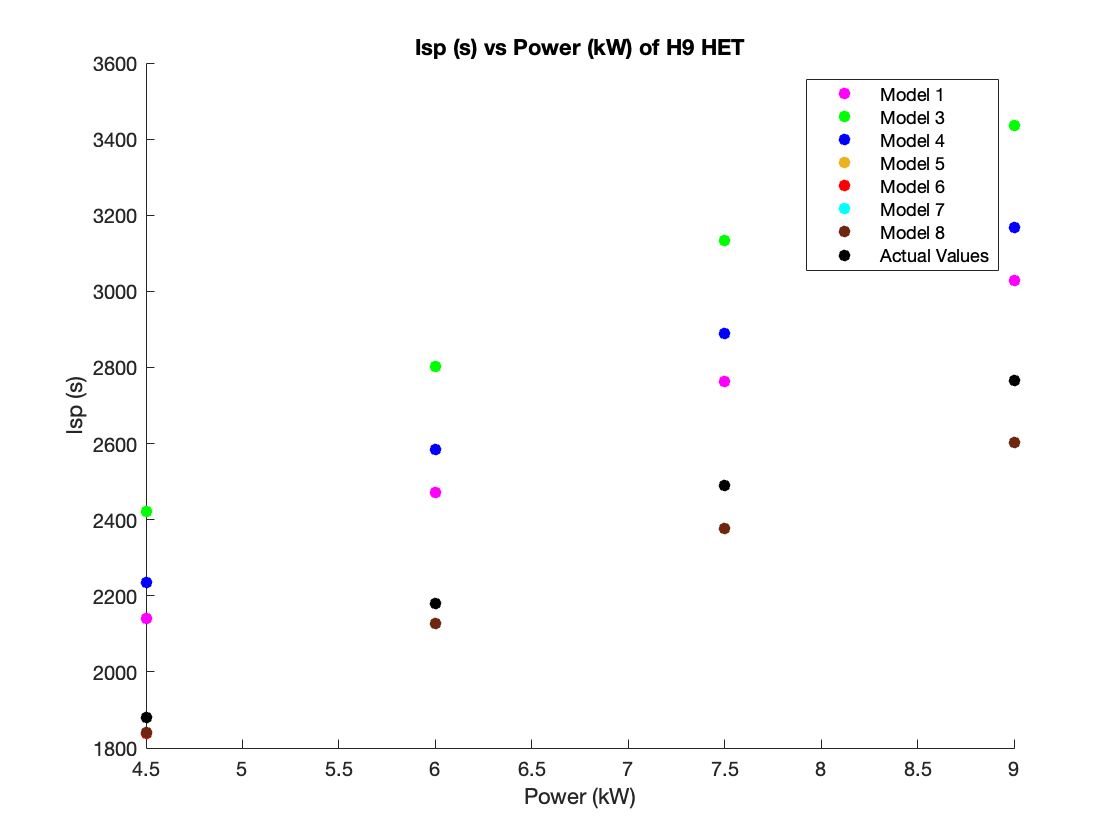
\includegraphics[width=3.3in]{Images/isp_vs_p.png}
      \caption{Graph of predicted efficiency values.}
      \label{fig:8}
\end{figure}

\begin{table}[H]
\centering
\begin{tabular}{ |c|c|c| }
 \hline
    Model & Thrust error (\%)  & $I_{sp}$ error (\%) \\
    \hline 
    \hline
    1 & 5.01\%  & 11.95\% \\
    \hline   
    3 & 10.69\%  & 18.07\% \\
    \hline   
    4 & 2.11\%  & 8.92\% \\
    \hline   
    5 & -7.34\%  & -10.42\% \\
    \hline   
    6 & -7.42\%  & -10.50\% \\
    \hline   
    7 & -0.36\%  & -3.72\% \\
    \hline   
    8 & -0.36\%  & -3.72\% \\
    \hline 
\end{tabular}
\caption{Average percent error for each model (Current fraction 80\%).}
\end{table}

\begin{table}[H]
\centering
\begin{tabular}{ |c|c|c| }
\hline
    Model & Thrust error (\%)  & $I_{sp}$ error (\%) \\
    \hline
    \hline
    1 & 5.01\%  & 11.95\% \\
    \hline   
    2 \& 3 & 18.98\%  & 26.85\% \\
    \hline   
    4 & 9.75\%  & 17.01\% \\
    \hline   
    5 & -0.42\%  & -3.78\% \\
    \hline   
    6 & -0.42\%  & -3.78\% \\
    \hline   
    7 & -0.36\%  & -3.72\% \\
    \hline  
    8 & -0.36\%  & -3.72\% \\
    \hline  
\end{tabular}
\par    
\caption{Average percent error for each model (Varying current fractions).}
\end{table}

Early models are severely lacking in accuracy. While they do follow the same trend as the real data, they have significant error. Therefore, it is inadvisable to use models other than 6, 7 and 8 for most applications. More than anything, earlier models reflect the process of creating accurate models rather than a tangible use case. 

Models 6 and 7/8 have different advantages. Model 6 does not offer improvements over Model 5; however, it requires fewer inputs which allows for the model to be applicable to more use cases where fewer initial data are known. Models 7 and 8, as they remove ion beam current as an input, are more accurate compared to all other models.

A simple way to get highly accurate thrust results from Model 6 is to predict the ion current fractions using Model 7, then running Model 6 with the new data. However, these current fractions are much higher than expected (.821 - .912). This points to a discrepancy in model equations, signaling potential room for improvement. Table 2 shows the error for data generated with the new current fractions.

\section{CONCLUSIONS}

In the end, the low percent error for thrust achieved by Models 7 and 8 is a success. Reducing this would still be ideal, as aerospace applications require very accurate simulations, and lighter weight numerical models can provide similar results. However, $I_{sp}$ error is much higher. While it is still sub-five percent, aerospace applications require very accurate predictions, and the $I_{sp}$ error is simply too high.

The increasing percent error for higher power simulations (visible on the graphs), while expected, is less than ideal. A current goal for HETs are increasing thrust to make them viable for more mission categories. Having an increasing error for higher power thrusters limits the usefulness of the models in a real-world setting for novel thruster design.

However, research into these models is still ongoing, and multiple avenues for model improvement remain open. Improving control volume analyses and looking at different forms of the efficiency ($I_{sp}$) equation (such as represented in \cite{c3})  are potential areas to concentrate efforts for future models on. Additionally, examining the cause of the difference between beam currents in literature and predicted values from my models is another area of potential focus.

Overall, while these techniques have proved fruitful in some areas, such as predicting thrust values, they are still lacking. Decreasing error in $I_{sp}$ values as well as decreasing the rise in error as HETs are simulated at higher power are requirements for this analytical modeling technique to be useful in real-world applications. 

\section*{ACKNOWLEDGMENT}

A massive thank you to my mentor, Charles Lipscomb, a PhD student at CU Boulder’s Nonequilibrium Gas and Plasma Dynamics Laboratory, for spending his time helping me accomplish this project. He was instrumental in making this project possible, from helping me learn the physics surrounding this project to assisting in drafting code and editing my writing. Thank you as well to Dr. Iain Boyd for connecting me with Charles and creating this opportunity. Additionally, thank you to Daniel Mydans for making the Research Seminar course at my high school possible.


%%%%%%%%%%%%%%%%%%%%%%%%%%%%%%%%%%%%%%%%%%%%%%%%%%%%%%%%%%%%%%%%%%%%%%%%%%%%%%%%


\begin{thebibliography}{99}

\bibitem{c1} King, Lyon B., and Alec D. Gallimore. Mass Spectral Measurements in the Plume of an SPT-100 Hall Thruster. [Accessed: 10- Dec- 2022].

\bibitem{c2} L. L. Su., \& B. A. Jorns (2021). Performance comparison of a 9-kW magnetically shielded Hall thruster operating on xenon and krypton. Available: \url{https://doi.org/10.1063/5.0066849}. [Accessed: 8- Apr- 2023].

\bibitem{c3} Hofer, Richard R., \& Robert S. Jankovsky (2001). A Hall Thruster Performance Model Incorporating the Effects of a Multiply-Charged Plasma. [Accessed: 10- Dec- 2022].

\bibitem{c4} Durot, Christopher J., et al (2017). Laser-Induced Fluorescence Measurement of the Anomalous Collision Frequency in a 9-kW Magnetically-Shielded Hall Thruster. [Accessed: 8- Apr- 2023].

\bibitem{c5} UMich PEPL. How Hall thrusters work (and why we can’t simulate them). [Online]. Available: \url{https://www.youtube.com/watch?v=mAfjmGMp43w}. [Accessed: 8- Apr- 2023].

\bibitem{c6} Doveil, F. \& Arcis, Nicolas \& Zurbach, S. (2012). Plasma propulsion for geostationary satellites for telecommunication and interplanetary missions. [Online]. Available: \url{https://www.researchgate.net/profile/F-Doveil/publication/254499071/figure/fig4/AS:668218632990732@1536327145607/View-of-a-Hall-Effect-Thruster-25.png}. [Accessed: 8- Apr- 2023].

\bibitem{c7} Williams, Matt (2022). The First Telescope Images of DART's Impact are Starting to Arrive. [Online]. Available: \url{https://www.universetoday.com/157812/the-first-telescope-images-of-darts-impact-are-starting-to-arrive/}. [Accessed: 8- Apr- 2023].

\bibitem{c8} Goebel, Dan M., \% Ira Gatz. Fundamentals of Electric Propulsion and Hall Thrusters. [Online]. Available: \url{https://descanso.jpl.nasa.gov/SciTechBook/series1/Goebel_02_Chap2_thruster.pdf}. [Accessed: 8- Apr- 2023].

\end{thebibliography}

\clearpage
\section*{APPENDIX}

\subsection{Model 8 Code:}

\begin{lstlisting}[language=Matlab]
    clear; clc
    
    syms gamma k Ta m m_dot A Va Vc q spec1 spec2 spec3 theta g
    syms ni vi1 vi2 vi3 vi I T Isp
    
    eq1 = m_dot == ni * vi * A * m * cosd(theta);
    
    eq3 = vi1 == sqrt(2 * 1 * q * (Va - Vc) / m);
    
    eq4 = vi2 == sqrt(2 * 2 * q * (Va - Vc) / m);
    
    eq5 = vi3 == sqrt(2 * 3 * q * (Va - Vc) / m);
    
    eq6 = vi == spec1 * vi1 + spec2 * vi2 + spec3 * vi3;
    
    eq8 = I == q * spec1 * ni * vi1 * A + 2 * q * spec2 * ni * vi2 * A + 3 * q * spec3 * ni * vi3 * A;
    
    eq9 = T == m_dot * vi * cosd(theta);
    
    eq10 = Isp == vi / g * cosd(theta);
    
    solution = solve([eq1, eq3, eq4, eq5, eq6, eq8, eq9, eq10], [ni, vi1, ...
        vi2, vi3, vi, I, T, Isp]);
    
    disp(simplify(solution.ni))
    disp(simplify(solution.vi1))
    disp(simplify(solution.vi2))
    disp(simplify(solution.vi3))
    disp(simplify(solution.vi))
    disp("I = ")
    disp(simplify(solution.I))
    disp("T = ")
    disp(simplify(solution.T))
    disp("Isp = ")
    disp(simplify(solution.Isp))
    
\end{lstlisting}

\subsection{Final Model Implementation Code:}

\begin{lstlisting}[language=Matlab]
    clear; clc
    
    %% Variable Definitions
    % thruster: h9
    g = 9.807; % acceleration due to gravity
    gamma = 5/3; % no units
    k = 1.380649e-23; % J/k
    Ta = 750; % kelvin (minor as all hell assumption)
    m = 2.1801714e-25; % kg
    m_dot = [14.8e-6, 15.4e-6, 16.4e-6, 15.4e-6]; % kg/s
    I = [15 * 0.821, 15 * 0.85646, 15 * 0.912, 15 * 0.856673]; % amps
    %I = [15 * 0.8, 15 * 0.8, 15 * 0.8, 15 * 0.8]; % amps
    A = .0645; % m^2
    Va = [300, 400, 500, 600]; % volts
    Vc = 0; % volts
    q = 1.602e-19; % one elementary charge in C
    spec1 = 0.888; % ion % w/ charge +1 (ASSUMPTION)
    spec2 = 0.110; % ion % w/ charge +2 (ASSUMPTION)
    spec3 = 0.002; % ion % w/ charge +3 (ASSUMPTION)
    theta = 25; % degrees (ASSUMPTION)
    real_isp = [1880, 2180, 2490, 2765]; % s
    real_thrust = [.295, .353, .417, .447]; % N
    power = [4.5, 6, 7.5, 9]; % kW
    thrust = zeros(8, numel(power)); % N
    isp = zeros(8, numel(power)); % s
    
    %% Data Generation
    for power_index = 1:numel(power)
        thrust(1, power_index) = T1(m_dot(power_index), q, Va(power_index), Vc, m);
        isp(1, power_index) = IspTMG(thrust(1, power_index), m_dot(power_index), g);
    
        thrust(3, power_index) = T3(gamma, k, Ta, m, m_dot(power_index), Va(power_index), Vc, q, I(power_index));
        isp(3, power_index) = IspTMG(thrust(3, power_index), m_dot(power_index), g);
    
        thrust(4, power_index) = T4(gamma, k, Ta, m, m_dot(power_index), Va(power_index), Vc, q, I(power_index), spec1, spec2, spec3);
        isp(4, power_index) = IspTMG(thrust(4, power_index), m_dot(power_index), g);
    
        thrust(5, power_index) = T5(gamma, k, Ta, m, m_dot(power_index), Va(power_index), Vc, q, I(power_index), spec1, spec2, spec3, theta);
        isp(5, power_index) = IspTMG(thrust(5, power_index), m_dot(power_index), g) * cosd(theta);
    
        thrust(6, power_index) = T6(gamma, k, Ta, m, Va(power_index), Vc, q, I(power_index), spec1, spec2, spec3, theta);
        isp(6, power_index) = IspTMG(thrust(6, power_index), m_dot(power_index), g) * cosd(theta);
        
        thrust(7, power_index) = T7(m, m_dot(power_index), Va(power_index), Vc, q, spec1, spec2, spec3, theta);
        isp(7, power_index) = IspTMG(thrust(7, power_index), m_dot(power_index), g) * cosd(theta);
    
        thrust(8, power_index) = T8(m, m_dot(power_index), Va(power_index), Vc, q, spec1, spec2, spec3, theta);
        isp(8, power_index) = IspTMG(thrust(8, power_index), m_dot(power_index), g) * cosd(theta);
    
    end
    
    %% Plot Generation
    
    figure()
    hold on
    title("Thrust (N) vs Power (kW) of H9 HET")
    scatter(power, thrust(1, :), 'magenta', 'filled')
    scatter(power, thrust(3, :), 'green', 'filled')
    scatter(power, thrust(4, :), 'blue', 'filled')
    scatter(power, thrust(5, :), 'filled', 'MarkerFaceColor', "#EDB120")
    scatter(power, thrust(6, :), 'red', 'filled')
    scatter(power, thrust(7, :), 'cyan', 'filled')
    scatter(power, thrust(8, :), 'filled', 'MarkerFaceColor', "#6E260E")
    scatter(power, real_thrust, 'black', 'filled')
    xlabel("Power (kW)")
    ylabel("Thrust (N)")
    legend(["Model 1", "Model 3", "Model 4", "Model 5", "Model 6", "Model 7", "Model 8", "Actual Values"])
    
    figure()
    hold on
    title("Isp (s) vs Power (kW) of H9 HET")
    scatter(power, isp(1, :), 'magenta', 'filled')
    scatter(power, isp(3, :), 'green', 'filled')
    scatter(power, isp(4, :), 'blue', 'filled')
    scatter(power, isp(5, :), 'filled', 'MarkerFaceColor', "#EDB120")
    scatter(power, isp(6, :), 'red', 'filled')
    scatter(power, isp(7, :), 'cyan', 'filled')
    scatter(power, isp(8, :), 'filled', 'MarkerFaceColor', "#6E260E")
    scatter(power, real_isp, 'black', 'filled')
    xlabel("Power (kW)")
    ylabel("Isp (s)")
    legend(["Model 1", "Model 3", "Model 4", "Model 5", "Model 6", "Model 7", "Model 8", "Actual Values"])
    
    %% Statistical Calculations
    error_percents = zeros(8, numel(power));
    
    % thrust
    for index = 1:numel(power)
        error_percents(1, index) = (thrust(1, index) - real_thrust(index)) / real_thrust(index) * 100.0;
        error_percents(3, index) = (thrust(3, index) - real_thrust(index)) / real_thrust(index) * 100.0;
        error_percents(4, index) = (thrust(4, index) - real_thrust(index)) / real_thrust(index) * 100.0;
        error_percents(5, index) = (thrust(5, index) - real_thrust(index)) / real_thrust(index) * 100.0;
        error_percents(6, index) = (thrust(6, index) - real_thrust(index)) / real_thrust(index) * 100.0;
        error_percents(7, index) = (thrust(7, index) - real_thrust(index)) / real_thrust(index) * 100.0;
        error_percents(8, index) = (thrust(8, index) - real_thrust(index)) / real_thrust(index) * 100.0;
    end
    
    error = mean(error_percents, 2);
    disp(error)
    
    % Isp
    for index = 1:numel(power)
        error_percents(1, index) = (isp(1, index) - real_isp(index)) / real_isp(index) * 100.0;
        error_percents(3, index) = (isp(3, index) - real_isp(index)) / real_isp(index) * 100.0;
        error_percents(4, index) = (isp(4, index) - real_isp(index)) / real_isp(index) * 100.0;
        error_percents(5, index) = (isp(5, index) - real_isp(index)) / real_isp(index) * 100.0;
        error_percents(6, index) = (isp(6, index) - real_isp(index)) / real_isp(index) * 100.0;
        error_percents(7, index) = (isp(7, index) - real_isp(index)) / real_isp(index) * 100.0;
        error_percents(8, index) = (isp(8, index) - real_isp(index)) / real_isp(index) * 100.0;
    end
    
    error = mean(error_percents, 2);
    disp(error)
    
    %% Function Definition
    function Isp = IspTMG(T, m_dot, g)
        Isp = T / (m_dot * g);
    end
    
    function T = T1(m_dot, q, Va, Vc, m)
        T = m_dot * sqrt(2 * q * (Va - Vc) / m);
    end
    
    function T = T3(gamma, k, Ta, m, m_dot, Va, Vc, q, I)
        T = -(I*Ta*gamma*k*m*((q*(Va - Vc))/m)^(1/2) - Ta*gamma*k*m_dot*q*((q*(Va - Vc))/m)^(1/2) - 2^(1/2)*I*Va*m*q*((Ta*gamma*k)/m)^(1/2) + 2^(1/2)*I*Vc*m*q*((Ta*gamma*k)/m)^(1/2))/(m*q*((q*(Va - Vc))/m)^(1/2)*((Ta*gamma*k)/m)^(1/2));
    end
    
    function T = T4(gamma, k, Ta, m, m_dot, Va, Vc, q, I, spec1, spec2, spec3)
        T = (2*I*Va*m*q*spec1*((Ta*gamma*k)/m)^(1/2) + 4*I*Va*m*q*spec2*((Ta*gamma*k)/m)^(1/2) + 6*I*Va*m*q*spec3*((Ta*gamma*k)/m)^(1/2) - 2*I*Vc*m*q*spec1*((Ta*gamma*k)/m)^(1/2) - 4*I*Vc*m*q*spec2*((Ta*gamma*k)/m)^(1/2) - 6*I*Vc*m*q*spec3*((Ta*gamma*k)/m)^(1/2) - 2*I*Ta*gamma*k*m*spec2*((q*(Va - Vc))/m)^(1/2) + 4*Ta*gamma*k*m_dot*q*spec2*((q*(Va - Vc))/m)^(1/2) - 2^(1/2)*I*Ta*gamma*k*m*spec1*((q*(Va - Vc))/m)^(1/2) - 6^(1/2)*I*Ta*gamma*k*m*spec3*((q*(Va - Vc))/m)^(1/2) + 2^(1/2)*Ta*gamma*k*m_dot*q*spec1*((q*(Va - Vc))/m)^(1/2) + 3*6^(1/2)*Ta*gamma*k*m_dot*q*spec3*((q*(Va - Vc))/m)^(1/2))/(m*q*((q*(Va - Vc))/m)^(1/2)*(4*spec2 + 2^(1/2)*spec1 + 3*6^(1/2)*spec3)*((Ta*gamma*k)/m)^(1/2));
    end
    
    function T = T5(gamma, k, Ta, m, m_dot, Va, Vc, q, I, spec1, spec2, spec3, theta)
        T = (4*Ta*gamma*k*m_dot*q*spec2*((q*(Va - Vc))/m)^(1/2) + 2*I*Va*m*q*spec1*cos((pi*theta)/180)*((Ta*gamma*k)/m)^(1/2) + 4*I*Va*m*q*spec2*cos((pi*theta)/180)*((Ta*gamma*k)/m)^(1/2) + 6*I*Va*m*q*spec3*cos((pi*theta)/180)*((Ta*gamma*k)/m)^(1/2) - 2*I*Vc*m*q*spec1*cos((pi*theta)/180)*((Ta*gamma*k)/m)^(1/2) - 4*I*Vc*m*q*spec2*cos((pi*theta)/180)*((Ta*gamma*k)/m)^(1/2) - 6*I*Vc*m*q*spec3*cos((pi*theta)/180)*((Ta*gamma*k)/m)^(1/2) + 2^(1/2)*Ta*gamma*k*m_dot*q*spec1*((q*(Va - Vc))/m)^(1/2) + 3*6^(1/2)*Ta*gamma*k*m_dot*q*spec3*((q*(Va - Vc))/m)^(1/2) - 2*I*Ta*gamma*k*m*spec2*cos((pi*theta)/180)*((q*(Va - Vc))/m)^(1/2) - 2^(1/2)*I*Ta*gamma*k*m*spec1*cos((pi*theta)/180)*((q*(Va - Vc))/m)^(1/2) - 6^(1/2)*I*Ta*gamma*k*m*spec3*cos((pi*theta)/180)*((q*(Va - Vc))/m)^(1/2))/(m*q*((q*(Va - Vc))/m)^(1/2)*(4*spec2 + 2^(1/2)*spec1 + 3*6^(1/2)*spec3)*((Ta*gamma*k)/m)^(1/2)); % N
    end
    
    function T = T6(gamma, k, Ta, m, Va, Vc, q, I, spec1, spec2, spec3, theta)
        T = (I*m*cos((pi*theta)/180)^2*((q*(Va - Vc))/m)^(1/2)*(2*spec2 + 2^(1/ ...
            2)*spec1 + 6^(1/2)*spec3)*(2*q*spec1*(Va - Vc)*((Ta*gamma*k)/m)^(1/ ...
            2) + 4*q*spec2*(Va - Vc)*((Ta*gamma*k)/m)^(1/2) + 6*q*spec3*(Va - ...
            Vc)*((Ta*gamma*k)/m)^(1/2) - 2*Ta*gamma*k*spec2*((q*(Va - Vc))/m)^ ...
            (1/2) - 2^(1/2)*Ta*gamma*k*spec1*((q*(Va - Vc))/m)^(1/2) - 6^(1/2)* ...
            Ta*gamma*k*spec3*((q*(Va - Vc))/m)^(1/2)))/(2*q^2*spec1^2*cos((pi* ...
            theta)/180)*(Va - Vc)*((Ta*gamma*k)/m)^(1/2) + 8*q^2*spec2^2*cos(( ...
            pi*theta)/180)*(Va - Vc)*((Ta*gamma*k)/m)^(1/2) + 18*q^2*spec3^2* ...
            cos((pi*theta)/180)*(Va - Vc)*((Ta*gamma*k)/m)^(1/2) - 4*Ta*gamma*k ...
            *q*spec2*((q*(Va - Vc))/m)^(1/2) + 6*2^(1/2)*q^2*spec1*spec2*cos(( ...
            pi*theta)/180)*(Va - Vc)*((Ta*gamma*k)/m)^(1/2) + 8*3^(1/2)*q^2* ...
            spec1*spec3*cos((pi*theta)/180)*(Va - Vc)*((Ta*gamma*k)/m)^(1/2) + ...
            10*6^(1/2)*q^2*spec2*spec3*cos((pi*theta)/180)*(Va - Vc)*((Ta*gamma ...
            *k)/m)^(1/2) - 2^(1/2)*Ta*gamma*k*q*spec1*((q*(Va - Vc))/m)^(1/2) - ...
            3*6^(1/2)*Ta*gamma*k*q*spec3*((q*(Va - Vc))/m)^(1/2));
    end
    
    function T = T7(m, m_dot, Va, Vc, q, spec1, spec2, spec3, theta)
        T = m_dot*cos((pi*theta)/180)*((q*(Va - Vc))/m)^(1/2)*(2*spec2 + 2^(1/2)*spec1 + 6^(1/2)*spec3); % N
    end
    
    function Isp = Isp8(theta, q, Va, Vc, m, spec1, spec2, spec3, g)
        Isp = (cos((pi*theta)/180)*((q*(Va - Vc))/m)^(1/2)*(2*spec2 + 2^(1/2)*spec1 + 6^(1/2)*spec3))/g;
    end
    
    function T = T8(m, m_dot, Va, Vc, q, spec1, spec2, spec3, theta)
        T = m_dot*cos((pi*theta)/180)*((q*(Va - Vc))/m)^(1/2)*(2*spec2 + 2^(1/2)*spec1 + 6^(1/2)*spec3); % N
    end
    
\end{lstlisting}

\end{document}
